\documentclass{beamer}

\usepackage[francais]{babel}
\usepackage[utf8]{inputenc}
\usepackage[T1]{fontenc}
\usepackage{graphicx}
\usepackage{graphics}
\usepackage{color}
\usepackage{textcomp}
\usepackage{pifont}
\usepackage[normalem]{ulem}
\usepackage{times}
\usepackage{hyperref}
\usepackage{verbatim}
\usepackage{amsmath}
\usepackage{amsthm}
\usepackage{amsfonts}
\usepackage[mathscr]{euscript}
\usepackage{pgfpages}
\usepackage{listings}
\usepackage{subfigure}
\usepackage{algorithm}
\usepackage[noend]{algorithmic}
\usepackage{pdftricks}
\usepackage{mathrsfs}
\usepackage{array}
\usepackage{fancybox}
% \usepackage{columns}
\usepackage{multirow}
\usepackage{url}
\usepackage{tikz}
\usepackage{colortbl}
%\usepackage{cite} %DO NOT FUCKING USE CITE ON BEAMER !!! LOST 30 GODDAM' MINUTES ON THIS SHIT !!!
\usepackage{mathabx}
\usepackage{amssymb}
\usepackage{eurosym}
\usepackage{wasysym} % ch0

\let\texteuro\euro

\hypersetup{colorlinks,%
            citecolor=black,%
            filecolor=black,%
            linkcolor=black,%
            urlcolor=blue}

%\addtolength{\parskip}{10pt}

\usetikzlibrary{calc}

\mode<presentation>
\setbeamertemplate{footline}[frame number]
\setbeamercovered{transparent}
\usetheme[navigation]{ESI}

%lst
\definecolor{comment-green}{RGB}{0,166,80}
\lstset{language=C++,
  keywordstyle=\lst@ifdisplaystyle\bf\fi\color{blue!60},
  commentstyle=\color{comment-green},
  stringstyle=\color{red},
  basicstyle=\lst@ifdisplaystyle\tiny\else\tt\fi,
  morekeywords={
    constexpr,concept,decltype,nullptr,nullptr_t,noexcept,final,override},
  frame=single,
  xleftmargin=0.5cm,
  numbers=left,
  tabsize=2}

%title
\subtitle{Langage \texttt{C} / \cpp}
\author{R. Absil}
\date{\today}

%styles
\theoremstyle{definition}
\newtheorem{thm}{Théorème}
\newtheorem{conj}[thm]{Conjecture}
\newtheorem{deff}[thm]{Définition}
\newtheorem{prop}[thm]{Propriété}
\newtheorem{lem}[thm]{Lemme}
\newtheorem*{lem*}{Lemme}
\newtheorem{cor}[thm]{Corollaire}
%\newtheorem{example}{Exemple}
\newtheorem{remark}{Remarque}
\newtheorem{exo}{Exercice}

%typeset
\newcommand{\ie}{{\emph{i.e., }}}
\newcommand{\eg}{{\emph{e.g., }}}
\newcommand{\etal}{{\emph{et al.}}}
\newcommand{\rrceil}{\unichar{"2308}}
\newcommand{\sloand}[2]{\footnote{N. J. A. Sloane - OEIS Foundation - \texttt{www.oeis.org}, Sequence #1 - #2.}}

%math
\newcommand{\IN}{{\mathbb N}}
\newcommand{\IQ}{{\mathbb Q}}
\newcommand{\IR}{{\mathbb R}}
\newcommand{\IZ}{{\mathbb Z}}
\newcommand{\IP}{{\mathbb P}}
\newcommand{\IC}{{\mathbb C}}
\newcommand{\bigo}{{\mathcal{O}}}
\renewcommand{\mod}{\bmod}
\newcommand{\ssi}{\Leftrightarrow}
\newcommand{\then}{\Rightarrow}
\newcommand{\fle}[1]{\stackrel{#1}{\longrightarrow}}
\newcommand{\suchthat}{~\big|~}
\newcommand{\floor}[1]{\left\lfloor #1 \right\rfloor}
\newcommand{\ceil}[1]{\left\lceil #1 \right\rceil}
\DeclareMathOperator*{\argmin}{argmin}
\DeclareMathOperator*{\argmax}{argmax}

%tikz
\tikzstyle{_vertex}=[fill=white, circle,minimum size=12pt,inner sep=1pt]
\tikzstyle{_blackv}=[fill=black, circle,minimum size=8pt,inner sep=1pt]
\tikzstyle{_dot}=[fill=black, circle, minimum size = 1mm, inner sep=0pt]
\tikzstyle{_bigvertex}=[fill=white, circle,minimum size=21pt,inner sep=1pt]
\tikzstyle{_arc}=[->, >=stealth]
\tikzstyle{_boldarc}=[->, >=stealth, line width=2pt]

\newcommand{\cpp}{\texttt{C++}}
\newcommand{\java}{\texttt{Java}}


\title{Ch. 11 - Conversions}

\begin{document}
\begin{frame}
  \titlepage
\end{frame}

\begin{frame}
  \frametitle{Table des matières}
  \footnotesize \tableofcontents[pausesections,pausesubsections]
\end{frame}


\section{Introduction}

\begin{frame}
\frametitle{\cpp\ et les conversions}
\begin{itemize}[<+->]
\item Pour les types de base en \texttt{C} / \cpp, les conversions ont déjà été abordées
\item Pour les autres types, en \cpp, il existe deux types de conversions
	\begin{enumerate}
	\item Explicites : demandées par l'utilisateur, via une instruction
	\item Implicites : mises en place automatiquement par le compilateur
	\end{enumerate}
\item Dans les deux cas, certaines conversions sont illégales
\end{itemize}
\begin{exampleblock}<+->{Opérateurs de conversion}
	\begin{itemize}[<+->]	
	\item \cpp\ : \lstinline|static_cast|, \lstinline|dynamic_cast|, \lstinline|reinterpret_cast|, \lstinline|const_cast|
	\item \texttt{C} : cast « régulier » (avec parenthèses)
		\begin{itemize}
		\item Combinaisons de casts \cpp\ (sans \lstinline|dynamic_cast|)
		\end{itemize}
	\end{itemize}
\end{exampleblock}
\end{frame}

\begin{frame}
\frametitle{Conversions explicites}
\begin{itemize}[<+->]
\item On a déjà vu plusieurs types de conversions explicites avec les types de base
\end{itemize}
\begin{exampleblock}<+->{Exemple}
	\begin{itemize}
	\item \lstinline|int n; double x;|
	\item \texttt{\{ ... \}}
	\item \lstinline|x = double(n);|
	\item \lstinline|n = int(x);|
	\end{itemize}
\end{exampleblock}
\begin{itemize}[<+->]
\item Conversions explicites, appelées avec l'opérateur de cast
	\begin{itemize}
	\item Toujours autorisé avec des types de base
	\item Tronquage possible
	\end{itemize}
\end{itemize}
\end{frame}

\begin{frame}
\frametitle{Conversions implicites}
\begin{itemize}[<+->]
\item « Non demandées » par l'utilisateur
\item Mises en place par le compilateur en fonction du contexte
\end{itemize}
\begin{exampleblock}<+->{Exemple}
	\begin{itemize}[<+->]
	\item Affectation : conversion dans le type de la variable réceptrice
	\item Appel de fonction : conversion d'un paramètre dans le type déclaré dans le prototype
	\item Au sein d'une expression : pour chaque opérateur, un opérande peut être convertie dans le type de l'autre
	\end{itemize}
\end{exampleblock}
\begin{itemize}[<+->]
\item Certaines conversions ne sont pas légales
	\begin{itemize}
	\item Celles qui impliquent des classes
	\item Pointeurs, sauf vers \lstinline|void*|
	\end{itemize}
\end{itemize}
\end{frame}

\begin{frame}
\frametitle{Conversions définies par l'utilisateur}
\begin{itemize}[<+->]
\item \cpp\ permet de définir soi-même des conversions implicites autorisées
\item Permet de faire implicitement des conversions de type
	\begin{enumerate}
	\item Classe $\rightarrow$ Type de base
	\item Type de base $\rightarrow$ Classe
	\item Classe $\rightarrow$ Classe
	\end{enumerate}
\item Mises en place via
	\begin{itemize}
	\item la surcharge d'un opérateur de cast
	\item l'écriture d'un constructeur « de conversion »
	\end{itemize}
\item Allège l'écriture de certains codes
\item Des conversions en chaîne peuvent avoir lieu
\end{itemize}
\end{frame}

\begin{frame}
\frametitle{Bonnes pratiques}
\begin{itemize}[<+->]
\item Les conversions définies par l'utilisateur peuvent s'avérer dangereuses
	\begin{itemize}[<+->]
	\item Le compilateur peut effectuer des conversions là où vous ne le voudriez pas
	\end{itemize}
\end{itemize}
\begin{block}<+->{Hygiène de programmation}
	\begin{itemize}[<+->]
	\item Ne pas abuser
	\item Écrire des conversions implicites « sensées »
	\end{itemize}
\end{block}
\begin{itemize}[<+->]
\item Exemple
	\begin{enumerate}[<+->]
	\item Oui : \texttt{fraction} $\rightarrow$ \lstinline|int|, \lstinline|int| $\rightarrow$ \texttt{fraction}
	\item Non : \lstinline|int| $\rightarrow$ \texttt{vector}, \texttt{vector} $\rightarrow$ \lstinline|int|
	\end{enumerate}
\end{itemize}
\end{frame}

\section{Conversions explicites}

\begin{frame}
\frametitle{Conversons explicites}
\begin{itemize}[<+->]
\item En \texttt{C} / \cpp, on a vu comment effectuer des conversions explicites entre types de base
	\begin{itemize}
	\item Avec un appel explicite à l'opérateur de cast
	\end{itemize}
\item En \cpp, il y a plusieurs autres types de conversions explicites
	\begin{enumerate}
	\item \lstinline|static_cast| : vérification à la compilation
	\item \lstinline|dynamic_cast| : vérification à l'exécution (polymotphisme) 
	\item \lstinline|const_cast| : supprime la cv-qualification
	\item \lstinline|reinterpret_cast| : conversion de motifs binaires
	\end{enumerate}
\item Le cast régulier effectue une combinaison des précédents, hors \lstinline|dynamic_cast|
\item Utiliser l'opérateur en fonction des besoins
\end{itemize}
\end{frame}

\begin{frame}
\frametitle{L'opérateur \texttt{static\_cast}}
\begin{itemize}[<+->]
\item Conversion avec vérification à la compilation
	\begin{itemize}
	\item \emph{Pas} à l'exécution
	\item Rapide
	\end{itemize}
\item Utilisation : \lstinline|static_cast<A>(b)|
	\begin{itemize}
	\item Convertit \texttt{b} vers un type \texttt{A}
	\end{itemize}
\item Permet
	\begin{itemize}
	\item « d'inverser » une conversion implicite
	\item d'effectuer un « downcast » dans le cas d'héritage
	\item d'effectuer des conversions tableaux $\rightarrow$ pointeurs, etc.
	\end{itemize}
\end{itemize}
\begin{block}<+->{Hygiène de programmation}
	\begin{itemize}[<+->]
	\item Utiliser au maximum quand on est certain du succès
		\begin{itemize}
		\item Vérification à l'exécution inutile
		\end{itemize}
	\end{itemize}
\end{block}
\end{frame}

\begin{frame}[containsverbatim]
\frametitle{Exemple}
\begin{itemize}
\item Fichier \texttt{static.cpp}
\end{itemize}
\begin{lstlisting}
int plusOne(void* pv)
{
	int * pi = static_cast<int*>(pv);
	(*pi)++; //ask why () are important
	return *pi;
}

struct B {}; //base class
struct D : B {}; //D inherits from B

int main()
{
	int i = 2;
	cout << plusOne(&i) << endl;
	cout << i << endl;

	D d;
	B& br = d; // upcast via implicit conversion
	D& another_d = static_cast<D&>(br); // manual downcast

	D a[10];
	B* dp = static_cast<B*>(a);//array to pointer + upcast
}
\end{lstlisting}
\end{frame}

\begin{frame}
\frametitle{L'opérateur \texttt{dynamic\_cast}}
\begin{itemize}[<+->]
\item Conversion avec vérification à l'exécution
	\begin{itemize}
	\item Plus lent que \lstinline|static_cast|
	\end{itemize}
\item Utilisation : \lstinline|dynamic_cast<A>(b)|
\item Pratique pour effectuer des conversions qui peuvent échouer
	\begin{itemize}
	\item downcast polymorphique	
	\end{itemize}
\item Si échec avec 
	\begin{itemize}
	\item un pointeur : retourne un \lstinline|nullptr|
	\item une référence : lance une exception \texttt{bad\_cast}
	\end{itemize}
\end{itemize}
\begin{block}<+->{Hygiène de programmation}
	\begin{itemize}[<+->]
	\item Utiliser pour conversions polymorphiques qui peuvent échouer
		\begin{itemize}
		\item Vérification à l'exécution indispensable
		\end{itemize}
	\end{itemize}
\end{block}
\end{frame}

\begin{frame}[containsverbatim]
\frametitle{Exemple}
\begin{itemize}
\item Fichier \texttt{dynamic.cpp}
\end{itemize}
\begin{lstlisting}
struct B 
{
    virtual void f() {};  // must be polymorphic to use runtime-checked dynamic_cast
};
struct D : B {}; //D inherits from A
 
int main()
{
    D d;
    B& b = d; //upcast
    D& new_d = dynamic_cast<D&>(b); // downcast
 
    B* b1 = new B;
    D* d1 = static_cast<D*>b1; //ok but D component is invalid
    if(D* d = dynamic_cast<D*>(b1))
    {
        std::cout << "downcast from b1 to d successful" << endl;
    }
 
    B* b2 = new D;
    if(D* d = dynamic_cast<D*>(b2))
    {
        std::cout << "downcast from b2 to d successful" << endl;
    }
}
\end{lstlisting}
\end{frame}

\begin{frame}
\frametitle{L'opérateur \texttt{const\_cast}}
\begin{itemize}[<+->]
\item Permet d'enlever la cv-qualification de pointeurs et références
	\begin{itemize}
	\item Ne fonctionne pas sur les pointeurs de fonctions
	\end{itemize}
\item Utilisation : \lstinline|const_cast<A>(b)|
\item Pratique si une référence (ou pointeur) est constant, mais pas l'objet référencé
\item Si la conversion échoue, le comportement est indéterminé
\end{itemize}
\begin{block}<+->{Hygiène de programmation}
	\begin{itemize}[<+->]
	\item Éviter d'écrire du code requérant un \lstinline|const_cast|
	\item Peu lisible, peut induire l'utilisateur en erreur
	\end{itemize}
\end{block}
\end{frame}

\begin{frame}[containsverbatim]
\frametitle{Exemple}
\begin{itemize}
\item Fichier \texttt{const.cpp}
\end{itemize}
\begin{lstlisting}
struct A 
{
    A() : i(3) {}
    void m1(int v) const 
    {
        // this->i = v;                 // compile error: this is a pointer to const
        const_cast<A*>(this)->i = v; // OK as long as the type object isn't const
    }
    int i;
};
 
int main() 
{
    int i = 3;               
    const int& cref_i = i; //const ref
    const_cast<int&>(cref_i) = 4; // OK: modifies i
    cout << "i = " << i << endl;
 
    A a;
    a.m1(4); //if a is const : undefined behaviour
    cout << "A::i = " << a.i << endl;
 
    const int j = 3; // j is declared const
    int* pj = const_cast<int*>(&j);
    *pj = 4;         // undefined behavior!
}
\end{lstlisting}
\end{frame}

\begin{frame}
\frametitle{L'opérateur \texttt{reinterpret\_cast}}
\begin{itemize}[<+->]
\item Permet de réinterpréter un motif binaire
\item Ne permet \emph{pas} de retirer la cv-qualification
\item Utilisation : \lstinline|reinterpret_cast<A>(b)|
\item Très dépendant de l'architecture
	\begin{itemize}
	\item Système little/big indian ?
	\end{itemize}
\item Souvent, peu de garanties sur le résultat
\end{itemize}
\begin{block}<+->{Hygiène de programmation}
	\begin{itemize}[<+->]
	\item Ne pas utiliser
	\end{itemize}
\end{block}
\end{frame}

\begin{frame}[containsverbatim]
\frametitle{Exemple}
\begin{itemize}
\item Fichier \texttt{reinterpret.cpp}
\end{itemize}
\begin{lstlisting}
struct A {  char a, b, c, d; };

int main()
{
    int i = 7;

    char* p2 = reinterpret_cast<char*>(&i);
    if(p2[0] == '\x7')
        cout << "This system is little-endian" << endl;
    else
        cout << "This system is big-endian" << endl;

    i = 1094861636; //0x41424344
    A &p = reinterpret_cast<A&>(i); //if little endian : D C B A

    cout << p.a << " " << p.b << " " << p.c << " " << p.d << endl;
}
\end{lstlisting}
\end{frame}

\begin{frame}
\frametitle{Le cast régulier}
\begin{itemize}[<+->]
\item Effectue une combinaisons des opérateurs précédents
	\begin{itemize}
	\item \emph{Pas} \lstinline|dynamic_cast|
	\end{itemize}
\item Le compilateur tente, dans cet ordre, d'effectuer
	\begin{enumerate}
	\item \lstinline|const_cast|
	\item \lstinline|static_cast|
	\item \lstinline|static_cast| suivi de \lstinline|const_cast|
	\item \lstinline|reinterpret_cast|
	\item \lstinline|reinterpret_cast| suivi de \lstinline|const_cast|
	\end{enumerate}
\end{itemize}
\begin{block}<+->{Hygiène de programmation}
	\begin{itemize}
	\item Éviter : utiliser \lstinline|static_cast| autant que possible
	\end{itemize}
\end{block}
\end{frame}

\begin{frame}
\frametitle{Le mot-clé \texttt{explicit}}
\begin{itemize}[<+->]
\item Empêche qu'un constructeur de conversion ou qu'un opérateur de cast soit utilisé lors de conversions implicites
\item \lstinline|explicit| sur un autre prototype provoque une erreur de compilation
\item Exemple dans le standard : constructeur de \texttt{vector}
	\begin{itemize}
	\item On en peut pas écrire \lstinline|vector<int> v = 2;|
	\end{itemize}
\item Pratique si l'on veut autoriser la conversion, mais que celle-ci est sujette à des erreurs si utilisée implicitement
	\begin{itemize}
	\item \lstinline|vector<int> v = 2;|
		\begin{itemize}
		\item vecteur de taille $2$, contenant deux zéros ?
		\item vecteur de taille $1$, contenant un unique $2$ ?
		\end{itemize}
	\item C'est une bonne pratique d'avoir défini ce constructeur comme \lstinline|explicit|
	\end{itemize}
\item Permet aussi de lever des ambiguïtés (cf. sections suivantes)
\end{itemize}
\end{frame}

\begin{frame}[containsverbatim]
\frametitle{Exemple}
\begin{itemize}
\item Fichier \texttt{explicit.cpp}
\end{itemize}
\begin{lstlisting}
struct B
{
    explicit B(int) {}
    explicit B(int, int) {}
    explicit operator int() const { return 0; }
};

int main()
{   
//  B b1 = 1; // Error
    B b2(2); // OK
    B b3 {4,5}; // OK
//  B b4 = {4,5}; // Error
//  int nb1 = b2; // Error
    int nb2 = static_cast<int>(b2); // OK
    B b5 = (B)1; // OK
}
\end{lstlisting}
\end{frame}

\section{Classe$\rightarrow$Type de base}

\begin{frame}
\frametitle{Définition}
\begin{itemize}[<+->]
\item Mis en place via la surcharge de l'opérateur de cast
\end{itemize}
\begin{exampleblock}<+->{Exemple : conversions vers \texttt{int}}
	\begin{itemize}[<+->]
	\item \lstinline|operator int() const \{ ... \}|
	\item Autorise des écritures 
		\begin{itemize}
		\item \lstinline|fraction f = ... ;|
		\item \lstinline|int n = f;|
		\end{itemize}
	\end{itemize}
\end{exampleblock}
\begin{itemize}[<+->]
\item Toujours défini comme une fonction membre
\item Le type de retour \emph{ne doit pas} être précisé
\end{itemize}
\end{frame}

\begin{frame}[containsverbatim]
\frametitle{Exemple}
\begin{itemize}
\item Fichier \texttt{fraction.cpp}
\end{itemize}
\begin{lstlisting}
class fraction
{
	unsigned num, denom;
	bool positive;

	public:
		fraction(int num, int denom) : ...
		{
			cout << "Call cstr " << num << " " << denom << endl;
		}		

		fraction(const fraction& f) : ...
		{
			cout << "Call copy cstr" << endl;
		}

		operator int() const
		{
			cout << "Call cast " << num << " " << denom << " " << positive << endl;
			return positive ? num / denom : -(num / denom); //ask why () needed
		}
};

void f1(int n) { cout << "Call f1(int) " << n << endl; }
void f2(double x) { cout << "Call f2(double) " << x << endl; }
\end{lstlisting}
\end{frame}

\begin{frame}[containsverbatim]
\frametitle{Exemple}
\begin{itemize}
\item Fichier \texttt{fraction.cpp}
\end{itemize}
\begin{lstlisting}
int main()
{
	fraction a(5,-2), b(2,5);
	int n1, n2;
	double x1, x2;
	cout << endl;

	n1 = int(a); cout << "n1 = " << n1 << endl;
	n2 = b; cout << "n2 = " << n2 << endl << endl;

	f1(a); f2(a);
	cout << endl;

	n1 = a + 3; cout << "n1 = " << n1 << endl;
	n2 = a + b; cout << "n2 = " << n2 << endl << endl;

	x1 = a + 3; cout << "x1 = " << x1 << endl;
	x2 = a + b; cout << "x2 = " << x2 << endl << endl;
	
	n1 = a + 3.85; cout << "n1 = " << n1 << endl;
	x1 = a + 3.85; cout << "x1 = " << x1 << endl;
	x2 = a; cout << "x2 = " << x2 << endl << endl;	
}
\end{lstlisting}
\end{frame}

\begin{frame}
\frametitle{Debriefing}
\begin{itemize}[<+->]
\item Plusieurs choses se produisent sur ce code
	\begin{itemize}
	\item Appel explicite et implicite de l'opérateur de cast à l'affectation
	\item Appel implicite de l'opérateur de cast lors de 
		\begin{itemize}
		\item l'appel de fonction
		\item l'évaluation d'une expression
		\end{itemize}
%	\item Conversions en chaîne \texttt{fraction} $\rightarrow$ \lstinline|int| $\rightarrow$ \lstinline|double|
	\end{itemize}
\end{itemize}
\begin{alertblock}<+->{Remarque}
	\begin{itemize}
	\item Aucun appel au constructeur de recopie n'est effectué
	\end{itemize}
\end{alertblock}
\begin{itemize}[<+->]
\item Évaluation \texttt{a + 3}
	\begin{enumerate}[<+->]
	\item Existe-t-il un opérateur \texttt{+} entre \texttt{fraction} et \lstinline|int| ?
	\item Existe-t-il des conversions possibles ?
		\begin{itemize}
		\item Conversion de \texttt{a} en \lstinline|int|
		\item Application de l'opérateur \texttt{+} entre \lstinline|int| et \lstinline|int|
		\end{itemize}
	\end{enumerate}
\end{itemize}
\end{frame}

\begin{frame}
\frametitle{Conversions en chaîne}
\begin{center}
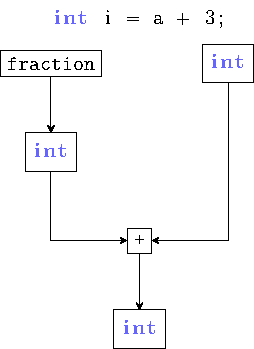
\includegraphics[height=6cm]{pics/conv-1.pdf}
\hspace{2cm}
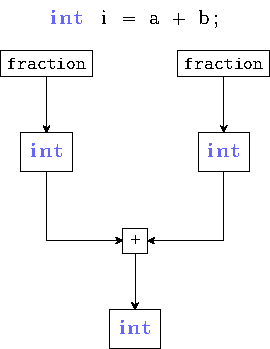
\includegraphics[height=6cm]{pics/conv-2.pdf}
\end{center}
\begin{itemize}
\item Plus de détails en fin de chapitre
\end{itemize}
\end{frame}

\section{Type de base$\rightarrow$Classe}

\begin{frame}
\frametitle{Définition}
\begin{itemize}[<+->]
\item Mis en œuvre via un constructeur à un paramètre
	\begin{itemize}
	\item Paramètres par défaut possible
	\item Si ambiguïté : rejet à la compilation
	\end{itemize}
\end{itemize}
\begin{exampleblock}<+->{Exemple}
	\begin{itemize}[<+->]
	\item \lstinline|fraction f = 12; //same as fraction f(12);|
	\end{itemize}
\end{exampleblock}
\begin{enumerate}[<+->]
\item Crée un objet temporaire de type \texttt{fraction}
\item Affecte cet objet à \texttt{f}
\end{enumerate}
\begin{itemize}[<+->]
\item Le compilateur accepte ce constructeur comme un « opérateur de conversion » de \lstinline|int| vers \texttt{fraction}
\end{itemize}
\end{frame}

\begin{frame}[containsverbatim]
\frametitle{Exemple}
\begin{itemize}
\item Fichier \texttt{fraction-2.cpp}
\end{itemize}
\begin{lstlisting}
class fraction
{
	...

	public:
		fraction(int num = 0, int denom = 1) : ...
		{
			cout << "Call cstr " << num << " " << denom << endl;
		}		

		fraction(const fraction& f) : ...
		{
			cout << "Call copy cstr" << endl;
		}
};

void f(fraction f) { cout << "Call f " << endl; }

int main()
{
	fraction fr(1,2);
	fr = fraction(3);
	fr = 12;
	f(5);
}
\end{lstlisting}
\end{frame}

\begin{frame}
\frametitle{Rappel sur les lvalue}
\begin{itemize}
\item Contraintes d'écriture, conversions, cv-qualifiers, règles d'appel, etc.
	\begin{itemize}
	\item Cf. Ch. 3 - Fonctions
	\end{itemize}
\end{itemize}
\begin{exampleblock}<+->{Conséquences}
	\begin{enumerate}[<+->]
	\item Si \texttt{f} avait été déclarée comme \lstinline|void f(fraction&)|, l'appel à \texttt{f(5)} aurait été rejeté à la compilation
	\item Si \texttt{f} avait été déclarée comme \lstinline|void f(const fraction&)|, l'appel à \texttt{f(5)} aurait été accepté
		\begin{enumerate}
		\item Conversion de \texttt{5} en \texttt{fraction}
		\item Création d'une fraction temporaire
		\item Transmission de la fraction par référence
		\end{enumerate}
	\end{enumerate}
\end{exampleblock}
\end{frame}

\begin{frame}[containsverbatim]
\frametitle{Choix entre constructeur et opérateur d'affectation}
\begin{itemize}
\item Fichier \texttt{fraction-3.cpp}
\end{itemize}
\begin{lstlisting}
class fraction
{
	unsigned num, denom;
	bool positive;

	public:
		fraction(int num = 0, int denom = 1) : ...
		{
			cout << "Call cstr " << num << " " << denom << endl;
		}	

		fraction& operator =(const fraction& f)
		{
			cout << "Aff. fraction " << f.num << " " << f.denom << " " << f.positive << endl;
			...
			return *this;
		}

		fraction& operator =(const int n)
		{
			cout << "Aff. int " << n << endl:
			...
			return *this;
		}	
};
\end{lstlisting}
\end{frame}

\begin{frame}
\frametitle{Règle de conversion}
\begin{exampleblock}<+->{Question}
	\begin{itemize}[<+->]
	\item Que fait une instruction \texttt{f = 12;} ?
	\end{itemize}
\end{exampleblock}
\begin{itemize}[<+->]
\item Deux choix possibles
	\begin{enumerate}
	\item Conversion \lstinline|int| $\rightarrow$ \texttt{fraction} suivi d'une affectation \texttt{fraction} $\rightarrow$ \texttt{fraction}
	\item Conversion \lstinline|int| $\rightarrow$ \texttt{fraction}
	\end{enumerate}
\end{itemize}
\begin{alertblock}<+->{Règle}
	\begin{itemize}[<+->]
	\item Les conversions définies par l'utilisateur, de type cast ou constructeur, ne sont mises en œuvre que lorsque cela est nécessaire
	\end{itemize}
\end{alertblock}
\end{frame}

\begin{frame}
\frametitle{Exemple d'utilisation : opérateurs arithmétiques}
\begin{itemize}[<+->]
\item Objectif : définir des opérateurs arithmétiques « symétriques »
\end{itemize}
\begin{exampleblock}<+->{Interface publique}
	\begin{itemize}
	\item \scriptsize{\lstinline|fraction::fraction(int n = 0, int num = 1);|}
	\item \scriptsize{\lstinline|fraction fraction::operator *(const fraction& f) const;|}
	\end{itemize}
\end{exampleblock}
\begin{alertblock}<+->{Problème}
	\begin{itemize}[<+->]
	\item On peut écrire \texttt{f * 2;} mais pas \texttt{2 * f;}
	\item Comme \texttt{*} est membre, le premier paramètre (\lstinline|this|) est toujours de type \texttt{fraction}
	\end{itemize}
\end{alertblock}
\end{frame}

\begin{frame}
\frametitle{Solution}
\begin{enumerate}[<+->]
\item Garder le constructeur « de conversion »
\item Définir \texttt{*} comme indépendant et amie de \texttt{fraction}
\end{enumerate}
\begin{exampleblock}<+->{Avantages}
	\begin{itemize}[<+->]
	\item Symétrie
	\item Efficace
	\item Permet de faire des chaînes de conversions
	\end{itemize}
\end{exampleblock}
\begin{itemize}[<+->]
\item Exemple avec constructeur de conversion de \lstinline|int|
	\begin{itemize}
	\item \lstinline|A * double|, \lstinline|A * int|, \lstinline|A * float|, \lstinline|A * long|, \lstinline|A * short|, \lstinline|A * char| et symétriques, etc.
	\end{itemize}
\end{itemize}
\end{frame}

\begin{frame}[containsverbatim]
\frametitle{Illustration}
\begin{itemize}
\item Fichier \texttt{fraction-4.cpp}
\end{itemize}
\begin{lstlisting}
class fraction
{
	unsigned num, denom;
	bool positive;

	public:
		fraction(int num = 0, int denom = 1) : ...
		{}				
    
        friend fraction operator * (fraction,fraction);
};

fraction operator *(fraction f1, fraction f2)
{
    return fraction(f1.num * f2.num, f1.denom * f2.denom);   
}
\end{lstlisting}
\end{frame}

\section{Classe$\rightarrow$Classe}

\begin{frame}
\frametitle{Définition}
\begin{itemize}[<+->]
\item Mis en œuvre soit via
	\begin{enumerate}
	\item la surcharge d'un opérateur de cast
	\item l'écriture d'un constructeur de conversion
	\end{enumerate}
\item Les règles d'application dans les conversions Classe $\rightarrow$ Type de bas et Type de base $\rightarrow$ Classe sont d'application
\item Les ambiguïtés sont rejetées à la compilation
	\begin{itemize}
	\item On ne peut pas utiliser les deux mécanismes
	\end{itemize}
\item La « qualité » de la conversion est laissée à la discrétion du programmeur
\end{itemize}
\end{frame}

\begin{frame}[containsverbatim]
\frametitle{Exemple cast}
\begin{itemize}
\item Fichier \texttt{fraction-5.cpp}
\end{itemize}
\begin{lstlisting}
class Fraction
{
	unsigned num, denom;
	bool positive;

	public:
		Fraction(int num, int denom) : ... {}

		operator ErrNbr();
};

class ErrNbr
{
	double f, error;	

	public:
		ErrNbr(double f, double error = 0) : f(f), error(error) {}	
		friend Fraction::operator ErrNbr();
};

Fraction::operator ErrNbr()
{
	return positive ? ErrNbr((num + 0.) / denom) : ErrNbr(-((num + 0.) / denom));
}
\end{lstlisting}
\end{frame}

\begin{frame}[containsverbatim]
\frametitle{Exemple constructeur}
\begin{itemize}
\item Fichier \texttt{fraction-6.cpp}
\end{itemize}
\begin{lstlisting}
class ErrNbr
{
	double f, error;	

	public:
		ErrNbr(double f, double error = 0) : f(f), error(error) {}
		ErrNbr(Fraction f);
};

class Fraction
{
	unsigned num, denom;
	bool positive;

	public:
		Fraction(int num, int denom) : ... {}
		friend ErrNbr::ErrNbr(Fraction);
};

ErrNbr::ErrNbr(Fraction f)  
	: f(f.positive ? (f.num + 0.) / f.denom : -((f.num + 0.) / f.denom)), error(0) {}
\end{lstlisting}
\begin{itemize}
\item Remarquez les différences dans les déclarations anticipées
\end{itemize}
\end{frame}

\section{Conversions en chaîne}

\begin{frame}
\frametitle{Conversions en chaîne}
\begin{exampleblock}<+->{Rappel}
	\begin{itemize}[<+->]
	\item Des conversions implicites en chaîne de types numériques sont effectuées
	\item Le compilateur privilégie les promotions numériques aux autres conversions
	\end{itemize}
\end{exampleblock}
\begin{itemize}[<+->]
\item En \cpp, le compilateur teste, dans cet ordre
	\begin{enumerate}
	\item Une conversion standard
	\item Une conversion définie par l'utilisateur
	\item Une conversion standard
	\end{enumerate}
\item Il est impossible d'effectuer en chaîne, implicitement, 
	\begin{itemize}
	\item deux conversions définies par l'utilisateur
	\item les trois actions ci-dessus
	\end{itemize}
\item Les ambiguïtés (deux chaînes possibles) sont rejetées à la compilation
\end{itemize}
\end{frame}

\begin{frame}[containsverbatim]
\frametitle{Conversion standard puis CDU}
\begin{itemize}
\item Fichier \texttt{chain1.cpp}
\end{itemize}
\begin{lstlisting}
class fraction 
{
	...
	
	public:
		fraction(int num = 0, int denom = 1) : ...
		{  }				

		explicit operator int() const
		{
			return positive ? num / denom : -(num / denom);
		}
    
		friend fraction operator * (fraction,fraction); 
};

int main()
{
	fraction f {1,2};  	    
	int i = static_cast<int>(f * 2.1);
}
\end{lstlisting}
\end{frame}

\begin{frame}
\frametitle{Illustration}
\begin{center}
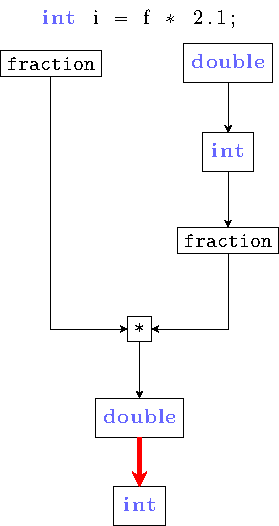
\includegraphics[height=6cm]{pics/conv-4.pdf}
\end{center}
\end{frame}

\begin{frame}[containsverbatim]
\frametitle{CDU puis conversion standard}
\begin{itemize}
\item Fichier \texttt{chain2.cpp}
\end{itemize}
\begin{lstlisting}
class fraction 
{
	...
	
	public:
		explicit fraction(int num = 0, int denom = 1) : ...
		{  }				

		operator int() const
		{
			return positive ? num / denom : -(num / denom);
		}
    
		friend fraction operator * (fraction,fraction); 
};

int main()
{
	fraction f {1,2};  	    
	int i = (f * 2.1);
}
\end{lstlisting}
\end{frame}

\begin{frame}
\frametitle{Illustration}
\begin{center}
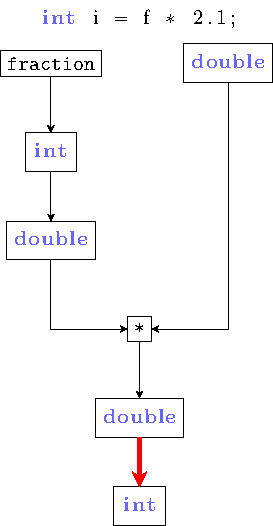
\includegraphics[height=6cm]{pics/conv-3.pdf}
\end{center}
\end{frame}

%\begin{frame}
%\frametitle{Illustration}
%\begin{center}
%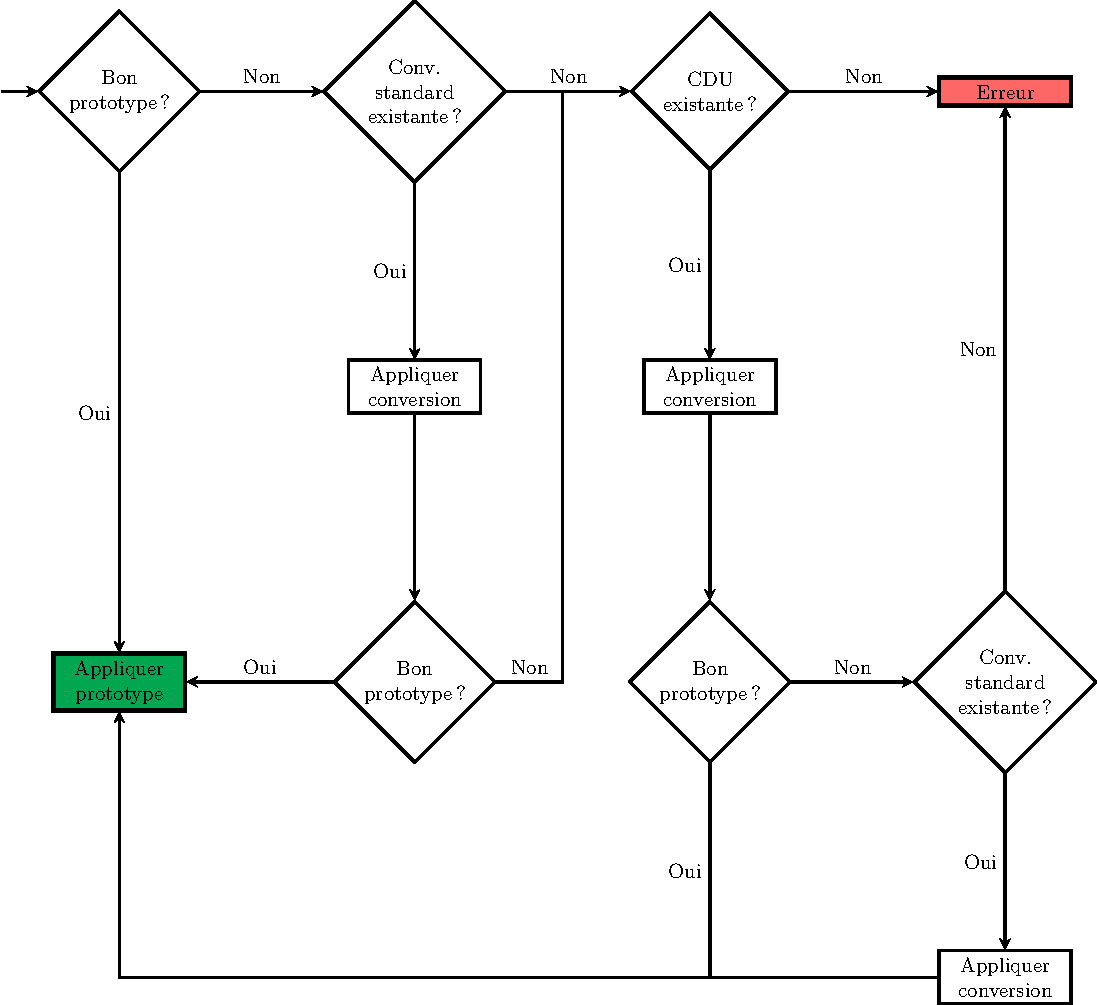
\includegraphics[height=.825\textheight]{pics/eval2.pdf}
%\end{center}
%\end{frame}

%\begin{frame}
%\frametitle{Contraintes}
%\begin{itemize}[<+->]
%\item À l'évidence, les ambiguïtés sont rejetées à la compilation
%\end{itemize}
%\begin{alertblock}<+->{Conséquence sur les conversions en chaîne}
%	\begin{itemize}[<+->]
%	\item Ne peuvent faire intervenir qu'une seule conversion définie par l'utilisateur
%	\item Formées au maximum de trois conversions 
%		\begin{enumerate}
%		\item Promotion
%		\item Conversion définie par l'utilisateur
%		\item Promotion
%		\end{enumerate}
%	\end{itemize}
%\end{alertblock}
%\end{frame}

\begin{frame}[containsverbatim]
\frametitle{Ambiguïté}
\begin{itemize}
\item Fichier \texttt{chain3.cpp}
\end{itemize}
\begin{lstlisting}
class fraction 
{
	...
	
	public:
		fraction(int num = 0, int denom = 1) : ...
		{  }				

		operator int() const
		{
			return positive ? num / denom : -(num / denom);
		}
    
		friend fraction operator * (fraction,fraction); 
};

int main()
{
	fraction f {1,2};  	    
	int i = (f * 2.1);
}
\end{lstlisting}
\end{frame}

\begin{frame}
\frametitle{Illustration}
\begin{center}
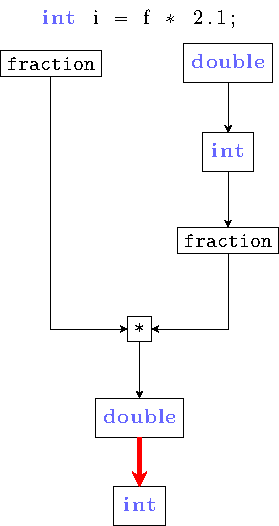
\includegraphics[height=5cm]{pics/conv-4.pdf}
\hspace{2cm}
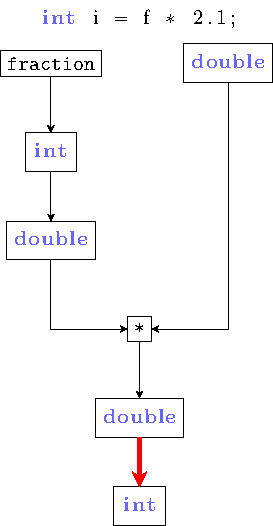
\includegraphics[height=5cm]{pics/conv-3.pdf}
\end{center}
\begin{itemize}
\item Utiliser \lstinline|explicit| là où, sémantiquement, on perd de la précision
	\begin{itemize}
	\item Ici, sur l'opérateur de cast (qui fait la division entière)
	\end{itemize}
\end{itemize}
\end{frame}

\begin{frame}[containsverbatim]
\frametitle{Autre exemple d'ambiguïté}
\begin{lstlisting}
class fraction
{
	explicit fraction(int n = 0, int denom = 1);
	operator int();
	operator double();	
};
\end{lstlisting}
\begin{lstlisting}
int i = f * 2.1;
\end{lstlisting}
\begin{center}
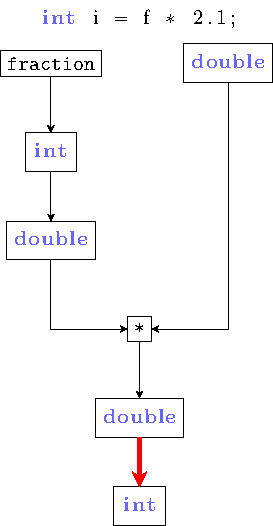
\includegraphics[height=4cm]{pics/conv-3.pdf}
\hspace{2cm}
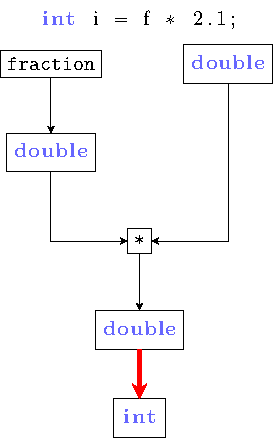
\includegraphics[height=4cm]{pics/conv-5.pdf}
\end{center}
\end{frame}
\end{document}
